\documentclass{article}
	\usepackage[utf8]{inputenc}
	\usepackage{float}
	\usepackage{pdfpages}
	\usepackage[T1]{fontenc}
	\usepackage{float}
	\usepackage{booktabs}
	\usepackage{multirow}
	\usepackage{ragged2e}
	\usepackage{makecell}
	\renewcommand{\theadfont}{\small\bfseries}
	\usepackage{tabularx}
	\usepackage[autolanguage, np]{numprint}
	\newcolumntype{Z}{ >{\centering\arraybackslash}X }
	\usepackage{makecell}
	\usepackage{url}
	\usepackage{siunitx}
	\usepackage{caption}
	\usepackage[framemethod=TikZ]{mdframed}
	\usepackage{tikz, tabularx}
	\usepackage[T1]{fontenc}
	\usepackage{charter}

%%% Document Properties and Packages used 9/20
\usepackage{amsmath}        % math formulas
\usepackage{bm}             % bold math symbols
\usepackage{multicol}       % multiple columns
\usepackage[super]{nth}     % 1st, 2nd, 3rd, 4th
\usepackage{enumitem}       % ordered list (a), (b), (c)
\usepackage{graphicx}		% insert images
\graphicspath{ {./images/} }
\usepackage{geometry}
\geometry{letterpaper, margin=1in, top=0.5in} % small margins
\usepackage{biblatex}		% bibliography
\addbibresource{HW1N1.bib}
%%%%%%%%%%%%%%%%%%%%%%%%%%%%%%%%%%%%%%%%%%%%%%%%%%%%%%%%%%%%%%%%%%%%%%%%%%%%%%%
%%% Code Listing 
\usepackage{listings}
\usepackage{xcolor}

\definecolor{codegreen}{rgb}{0,0.6,0}
\definecolor{codegray}{rgb}{0.5,0.5,0.5}
\definecolor{codepurple}{rgb}{0.58,0,0.82}
\definecolor{backcolour}{rgb}{0.95,0.95,0.92}

\lstdefinestyle{mystyle}{
	backgroundcolor=\color{backcolour},   
	commentstyle=\color{codegreen},
	keywordstyle=\color{magenta},
	numberstyle=\tiny\color{codegray},
	stringstyle=\color{codepurple},
	basicstyle=\ttfamily\footnotesize,
	breakatwhitespace=false,         
	breaklines=true,                 
	captionpos=b,                    
	keepspaces=true,                 
	numbers=left,                    
	numbersep=5pt,                  
	showspaces=false,                
	showstringspaces=false,
	showtabs=false,                  
	tabsize=2
}
\lstset{style=mystyle}
%%%%%%%%%%%%%%%%%%%%%%%%%%%%%%%%%%%%%%%%%%%%%%%%%%%%%%%%%%%%%%%%%%%%%%%%%%%%%%%
\begin{document}
	
	\noindent\textbf{Justine John "JJ" A. Serdoncillo}
	\hfill \textbf{AEM 5253: Computational Fluid Dynamics} \\ \hfill \textbf{October 10, 2022}
	
	\begin{center}
		\Large{\textbf{Homework 1}}    
	\end{center}
	
	\section*{Number 1 a)}
		Calculating the analytical solution we find:
		\begin{align*}
			   \frac{dy}{dt} 		& = -2y
			\\ \int \frac{dy}{y} 	& = \int -2 dt
			\\ [ln|y|]^{y}_{y_0}	& = -2t
			\\ ln|\frac{y}{y_0}|	& = -2t
			\\ \frac{y}{y_0}		& = -2t
		\end{align*}
		$$ \makebox{\fbox{  y = y_0 e^{-2t} = 4 e^{-2t} }} $$
		\noindent
		Using the code used in the appendix, the following plots were made below.
		\begin{figure}[H]
			\centering
			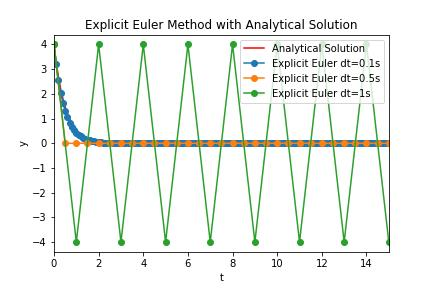
\includegraphics[width=0.8\textwidth]{images/exp1a.jpg}
			\caption{\label{} Explicit Euler at different time steps}
		\end{figure}
		From the figure above it can be seen that all of the different time steps were stable. However, the largest time step's output oscillates between 4 and -4 which doesn't help depict the actual solution. It seems to be the critical time step between stability and unstability. For the medium time step, it immediately jumped to 0 and became it's steady state value which is somewhat true but doesn't show the details of the exponential function. The smallest time step accurately depicts the analytical equation properly. 
		\begin{figure}[H]
			\centering
			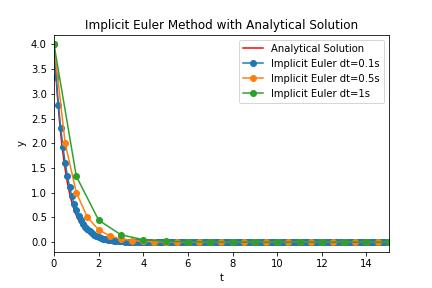
\includegraphics[width=0.8\textwidth]{images/imp1a.jpg}
			\caption{\label{} Implicit Euler at different time steps}
		\end{figure}
		For the implicit euler method, all of the time steps were all seemingly accurate and stable. It's accuracy increased as the time step decreased and was even almost on top of the exact solution for the smallest time step. 
		\begin{figure}[H]
			\centering
			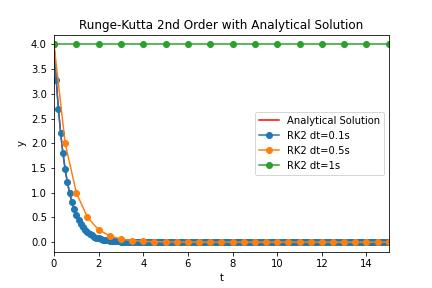
\includegraphics[width=0.8\textwidth]{images/rk21a.jpg}
			\caption{\label{} Runge-Kutta \nth{2} order at different time steps}
		\end{figure}
		For the \nth{2} order Runge-Kutta method, the plots are similar to the implicit euler except for the largest time step. It seemed like it is stable but only hovers at 4 which doesn't explain the analytical solution whatsoever. 
		\begin{figure}[H]
			\centering
			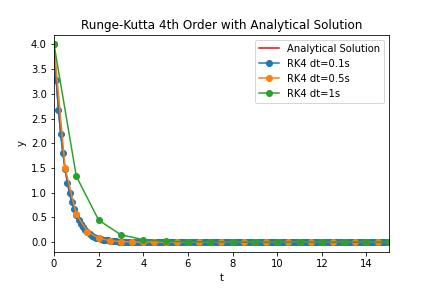
\includegraphics[width=0.8\textwidth]{images/rk41a.jpg}
			\caption{\label{} Runge-Kutta \nth{4} order at different time steps}
		\end{figure}
		The \nth{4} order Runge-Kutta method all have the plots stable and accurate for the different time steps. Comparing with the implicit euler method, it can be seen that it does not perform as well with the largest time step but does better in the medium time step.
	
	\section*{Number 1 b)}
		Using the model equation $\frac{dy}{dt} = g(y,t) = cy$ to the given equation. It can be found that $c=-2$. The critical time step for stable but oscillating can be found by forcing $-1 \leq \sigma \leq 0$ .
		\begin{enumerate}[label=(\alph*)]
			\item Explicit Euler: 
				$$\frac{y_{n+1}-y_n}{\Delta t} = -2y_n $$
				$$y_{n+1} = y_{n} - 2\Delta t y_{n}$$
				$$y_{n+1} = y_{n}(1 - 2\Delta t)$$
				$$\sigma = (1-2\Delta t)$$
				$$-1 \leq 1-2\Delta t \leq 0$$
				$$-2 \leq -2\Delta t \leq -1$$
				$$1 > \Delta t > \frac{1}{2}$$
				$$ \frac{1}{2} < \Delta t < 1  $$
				critical time step at \makebox{\fbox{ $\Delta t = \frac{1}{2}$  }}  			
			\item Implicit Euler:
				$$\frac{y_{n+1}-y_n}{\Delta t} = -2y_{n+1} $$
				$$y_{n+1} = \frac{y_n}{1+2\Delta t}$$
				$$\sigma = \frac{1}{1+2\Delta t}$$
				$$-1 \leq \frac{1}{1+2\Delta t} \leq 0 $$
				$$ -1-2\Delta t \leq 1 $$
				$$ -2 \Delta t \leq 2 $$
				$$ -1 < \Delta t $$
				\makebox{\fbox{ no critical time step  }}  	
			\item Runge-Kutta \nth{2} order:
				$$y_{n+1} = y_{n} (1+c\Delta t + \frac{1}{2} (c\Delta t)^2) $$
				$$\sigma = 1+c\Delta t + \frac{1}{2} (c\Delta t)^2  $$
				$$\sigma = 1-2\Delta t + \frac{1}{2} (-2\Delta t)^2 $$
				$$ 0 \leq 1-2\Delta t + 2\Delta t^2 \leq -1 $$
				from here it can be seen that there is no critical time step for oscillation yet stable
				$$| 1-2\Delta t + 2\Delta t^2 | \leq 1 $$
				$$ -1 \leq 1-2\Delta t + 2\Delta t^2 \leq 1 $$
				solving from both sides 
				$$ 0 < \Delta t < 1 $$
				critical time step at \makebox{\fbox{ $\Delta t = 1$  }}  	
			\item Runge-Kutta \nth{4} order:
				$$y_{n+1} = y_{n} (1+c\Delta t + \frac{1}{2} (c\Delta t)^2 + \frac{1}{6} (c\Delta t)^3 + \frac{1}{24} (c\Delta t)^4) $$
				$$\sigma = 1+c\Delta t + \frac{1}{2} (c\Delta t)^2 + \frac{1}{6} (c\Delta t)^3 + \frac{1}{24} (c\Delta t)^4  $$
				$$\sigma = 1-2\Delta t + \frac{1}{2} (-2\Delta t)^2 + \frac{1}{6} (-2\Delta t)^3 + \frac{1}{24} (-2\Delta t)^4 $$
				$$-1 \leq 1-2\Delta t + 2\Delta t^2 -\frac{4}{3} \Delta t^3 + \frac{2}{3} \Delta t^4  \leq 0 $$
				from here it can be seen that there is no critical time step for oscillation yet stable
				$$| 1-2\Delta t + 2\Delta t^2 -\frac{4}{3} \Delta t^3 + \frac{2}{3} \Delta t^4 | \leq 1 $$
				solving for $\Delta t$ we get
				$$ 0 < \Delta t < 1.393 $$
				critical time step at \makebox{\fbox{ $\Delta t = 1.393$  }}  	
		\end{enumerate}
	
	\section*{Number 2 a)}
		Using the model equation $\frac{dy}{dt} = g(y,t) = cy$ to the given equation. It can be found that $c=-(2+0.01^2)$. The estimated maximum stable time step over the entire domain of interest can be found by forcing $\sigma \leq 1$ and $t \leq 15 $.
		\begin{enumerate}[label=(\alph*)]
			\item Explicit Euler: 
			$$\frac{y_{n+1}-y_n}{\Delta t} = -(2+0.01t^2)y_n $$
			$$y_{n+1} = y_{n} -(2+0.01t^2)\Delta t y_{n}$$
			$$y_{n+1} = y_{n}(1 -(2+0.01t^2)\Delta t)$$
			$$\sigma = (1-(2+0.01t^2)\Delta t)$$
			$$|1-(2+0.01t^2)\Delta t| \leq 1$$
			$$-1 \leq 1-(2+0.01t^2)\Delta t \leq 1$$
			$$-2 \leq -(2+0.01t^2)\Delta t $$
			$$ -(2+0.01t^2)\Delta t < 2  $$
			$$ \Delta t < \frac{1}{1+0.005t^2}$$
			as $t \rightarrow \infty$, $\frac{1}{1+0.005t^2}$ decreases. To get the maximum stable time step, we minimize the value which occurs at $t = 0$ \\
			Estimated maximum stable time step at \makebox{\fbox{ $\Delta t = 1$  }}  			
			\item Implicit Euler:
			$$\frac{y_{n+1}-y_n}{\Delta t} = -(2+0.01t^2)y_{n+1} $$
			$$y_{n+1} = \frac{y_n}{1+(2+0.01t^2)\Delta t}$$
			$$\sigma = \frac{1}{1+(2+0.01t^2)\Delta t}$$
			$$| \frac{1}{1+(2+0.01t^2)\Delta t} |\leq 1 $$
			$$ \frac{1}{1+(2+0.01t^2)\Delta t} \leq 1 $$
			$$ 1 \leq 1 + (2+0.01t^2)\Delta t $$
			$$ 0 \leq (2+0.01t^2)\Delta t $$
			$2+0.01 t^2$ is always greater than 0, hence
			$$ 0 \leq \Delta t $$
			\makebox{\fbox{ no critical time step  }}  	
			\item Runge-Kutta \nth{2} order:
				$$y_{n+1} = y_{n} (1+c\Delta t + \frac{1}{2} (c\Delta t)^2) $$
				$$\sigma = 1+c\Delta t + \frac{1}{2} (c\Delta t)^2  $$
				$$\sigma = 1-(2+0.01t^2)\Delta t + \frac{1}{2} (-(2+0.01t^2)\Delta t)^2 $$
				
				$$| 1-(2+0.01t^2)\Delta t + \frac{1}{2}(2+0.01t^2)^2\Delta t^2 | \leq 1 $$
				By evaluating at different values of $t$ it can be seen that the maximum $\Delta t$ also changes. At $t=15$ the maximum stable time step is $\Delta t=0.471$, however at $t=0$ the maximum stable time step is $\Delta t=1$. Taking the higher value of the two, the estimated maximum stable time step at \makebox{\fbox{ $\Delta t = 1$  }} 
			\item Runge-Kutta \nth{4} order:
				$$y_{n+1} = y_{n} (1+c\Delta t + \frac{1}{2} (c\Delta t)^2 + \frac{1}{6} (c\Delta t)^3 + \frac{1}{24} (c\Delta t)^4) $$
				$$\sigma = 1+c\Delta t + \frac{1}{2} (c\Delta t)^2 + \frac{1}{6} (c\Delta t)^3 + \frac{1}{24} (c\Delta t)^4  $$
				
				$$\sigma = 1-(2+0.01t^2)\Delta t + \frac{1}{2} (-(2+0.01t^2)\Delta t)^2 + \frac{1}{6} (-(2+0.01t^2)\Delta t)^3 + \frac{1}{24} (-(2+0.01t^2)\Delta t)^4 $$
				$$| 1-(2+0.01t^2)\Delta t + \frac{1}{2} (-(2+0.01t^2)\Delta t)^2 + \frac{1}{6} (-(2+0.01t^2)\Delta t)^3 + \frac{1}{24} (-(2+0.01t^2)\Delta t)^4 | \leq 1 $$
				Using the same thought process as for the previous scheme, at $t=15$ the maximum stable time step is $\Delta t=0.348$, however at $t=0$ the maximum stable time step is $\Delta t=0.74$. Taking the higher value of the two, the estimated maximum stable time step at \makebox{\fbox{ $\Delta t = 0.74$  }} 
		\end{enumerate}
	
	\section*{Number 2 b)}
		Calculating the analytical solution we find:
		\begin{align*}
			\frac{dy}{dt} 		& = -(2+0.01t^2)y
			\\ \int \frac{dy}{y} 	& = \int -(2+0.01t^2) dt
			\\ [ln|y|]^{y}_{y_0}	& = -(2t+\frac{0.01}{3}t^3)
			\\ ln|\frac{y}{y_0}|	& = -(2t+\frac{0.01}{3}t^3)
			\\ \frac{y}{y_0}		& = -(2t+\frac{0.01}{3}t^3)
		\end{align*}
		$$ \makebox{\fbox{  y = y_0 e^{-(2t+\frac{0.01}{3}t^3)} = 4 e^{-(2t+\frac{0.01}{3}t^3)} }} $$
		\noindent
		The implicit solution can be derived by taking two equations with two unknowns. More can be seen in the code below. \\
		Using the code used in the appendix, the following plots were made below.
		\begin{figure}[H]
			\centering
			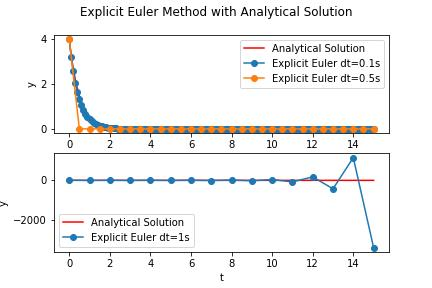
\includegraphics[width=0.8\textwidth]{images/exp2a.jpg}
			\caption{\label{} Explicit Euler at different time steps}
		\end{figure}
		Similar with the case with the previous problem, the largest time step was unstable and the medium time step, although stable quickly moved to near 0 which lost the details for the actual solution. The smallest time step is both stable and accurate.
		\begin{figure}[H]
			\centering
			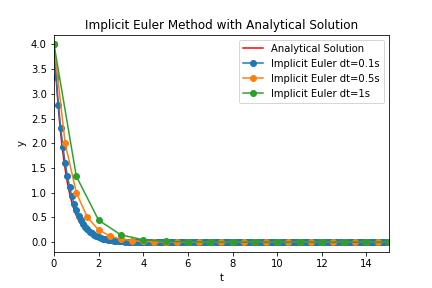
\includegraphics[width=0.8\textwidth]{images/imp2a.jpg}
			\caption{\label{} Implicit Euler at different time steps }
		\end{figure}
		For implicit euler, all of the plots were stable and getting more accurate as the time step decreased.
		\begin{figure}[H]
			\centering
			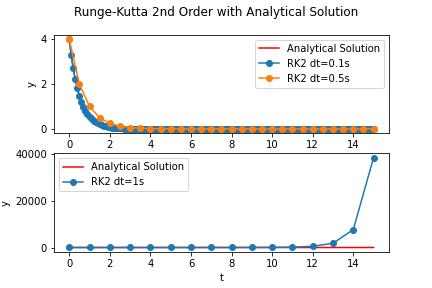
\includegraphics[width=0.8\textwidth]{images/rk22a.jpg}
			\caption{\label{} Runge-Kutta \nth{2} order at different time steps}
		\end{figure}
		The plots showed to be stable for the first two time steps but was unstable in the largest time step. 
		\begin{figure}[H]
			\centering
			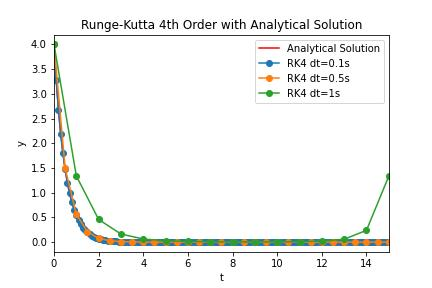
\includegraphics[width=0.8\textwidth]{images/rk42a.jpg}
			\caption{\label{} Runge-Kutta \nth{4} order at different time steps}
		\end{figure}
		For the Runge-Kutta \nth{4} order method, it seemed like all of the plots were somewhat accurate within the range of the domain but the largest time step showed signs of instability near the end. 
	
	\section*{Number 3 a)}
		Linearizing the second order equation, the following is derived below
		$$ \frac{d\theta}{dt} = \dot{\theta} \quad \mathrm{and} \quad \frac{d\dot{\theta}}{dt} = -\frac{g}{l} \theta  $$
		or converted into matrices
		$$\frac{d}{dt} \begin{bmatrix}\theta \\ \dot{\theta} \end{bmatrix} = \begin{bmatrix} 0 & 1 \\ -\frac{g}{l} & 0 \end{bmatrix} \begin{bmatrix}\theta \\ \dot{\theta} \end{bmatrix} $$
		Using the code used in the appendix, the following plots were made below.
		\begin{figure}[H]
			\centering
			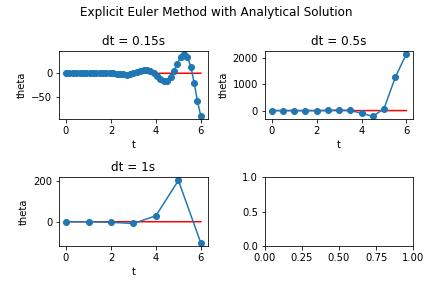
\includegraphics[width=0.8\textwidth]{images/exp3a.jpg}
			\caption{\label{} Explicit Euler at different time steps}
		\end{figure}
		From the figure above which uses the explicit Euler method, it can be seen that the plots of all of the different time steps are neither accurate nor stable. At the smallest time step, the first few values might be accurate enough but the oscillation grew larger and deviated from the exact solution.
		\begin{figure}[H]
			\centering
			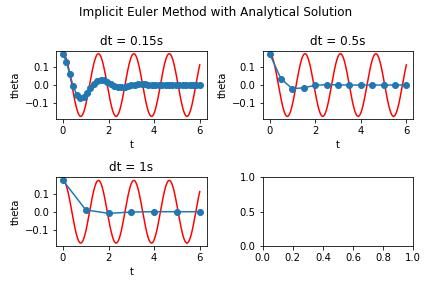
\includegraphics[width=0.8\textwidth]{images/imp3a.jpg}
			\caption{\label{} Implicit Euler at different time steps }
		\end{figure}
		For the implicit scheme, the case is different as all of the plots of the different timesteps were all stable. However, looking at the figure, it can be seen that neither of these looks even close to the exact solution.
		\begin{figure}[H]
			\centering
			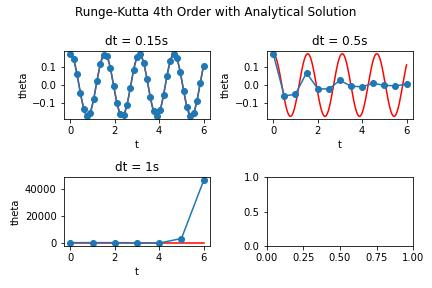
\includegraphics[width=0.8\textwidth]{images/rk43a.jpg}
			\caption{\label{} Runge-Kutta \nth{4} order at different time steps}
		\end{figure}
		Lastly for the Runge-Kutta $\nth{4}$ order method, the figures were stable for the first two time steps. In the case of accuracy, the second time step was not accurate in representing the exact solution but showed an oscillatory though. The smallest time step looks to be both stable and 
	\section*{Number 3 b)}
		Using the code used in the appendix, the following plots were made below.
		\begin{figure}[H]
			\centering
			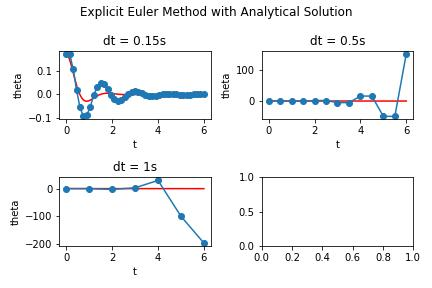
\includegraphics[width=0.8\textwidth]{images/exp3b.jpg}
			\caption{\label{} Explicit Euler at different time steps}
		\end{figure}
		From the figure above, it can be seen that the explicit euler method showed to be stable in the smallest timestep. Even though it didn't match the frequency of the oscillation nor the damping right, there was a damped motion that can be seen and that the value rose at almost the same time step as with the exact solution. For the other time steps, it can be seen that they are unstable. For the second time step, the oscillation was growing rather than decreasing while for the last time step, the oscillation is barely seen.
		\begin{figure}[H]
			\centering
			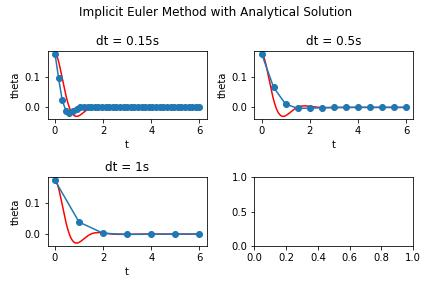
\includegraphics[width=0.8\textwidth]{images/imp3b.jpg}
			\caption{\label{} Implicit Euler at different time steps }
		\end{figure}
		For the implict euler method, all of the time steps showed to be stable and even approached the right steady state solution. However it's accuracy seems to be highly compromised because in the largest time step, there seems to be no damping seen and barely noticeable in the medium time step. In the smallest time step however, it can be seen to mimic the trend of the exact solution but not accurately enough.
		\begin{figure}[H]
			\centering
			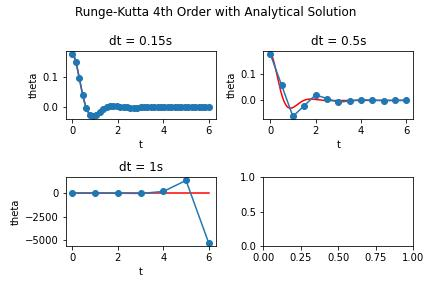
\includegraphics[width=0.8\textwidth]{images/rk43b.jpg}
			\caption{\label{} Runge-Kutta \nth{4} order at different time steps}
		\end{figure}
		Lastly for the Runge-Kutta method, it can be seen that the largest time time is unstable and doesn't seem to be accurate as well. In the medium time step, it was stable and that some of the points were close to the actual value and it showed the damped response in the actual solution. For the smallest time step, it can be seen that it accurately depicted the actual solution and also stable as well. 
	\section*{Number 4 a)}
		\begin{figure}[H]
			\centering
			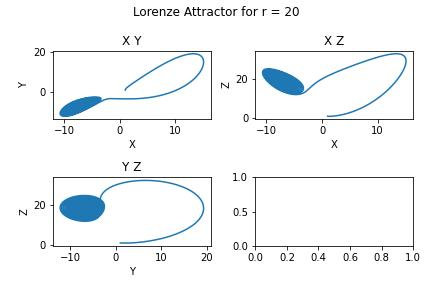
\includegraphics[width=0.8\textwidth]{images/rk44a.jpg}
			\caption{\label{} Lorenz attractor at r=20 starting at (1,1,1) }
		\end{figure}
		The figure above shows the plot of the attractor in all planes and it can be seen that the figures are stable and approach a specific domain in space.
	\section*{Number 4 b)}
		\begin{figure}[H]
			\centering
			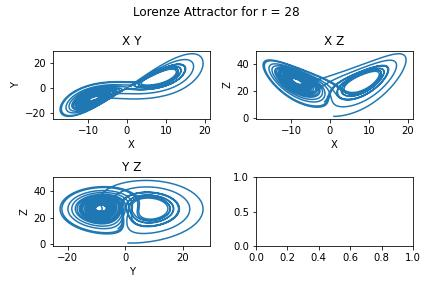
\includegraphics[width=0.8\textwidth]{images/rk44b.jpg}
			\caption{\label{} Lorenz attractor at r=28 starting at (1,1,1)}
		\end{figure}
		As the value of $r$ was increased beyond its limit, it can be seen that the plot now goes around in space a lot more and seems to be orbiting between two different areas in space. It does seem to still be confined in a specific domain and does not blow up to much higher values. 
	\section*{Number 4 c)}
		\begin{figure}[H]
		\centering
		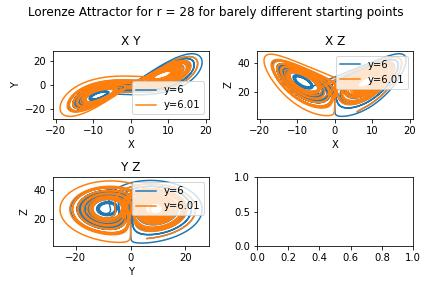
\includegraphics[width=0.8\textwidth]{images/rk44c.jpg}
		\caption{\label{} Lorenz attractor at r=28 with two different starting point at (6,6,6) and (6,6.01,6)}
		\end{figure}
		By only changing $y$ by 0.01, it can be seen that from the figure above that the plot changed drastically. Both of the figures have a similar trend and movement that is also close to the attractor from the previous section but it is distinct enough from each other that the plots can be seen separately. 
	
	\section*{Number 5 a)}
		Using the code used in the appendix below. A following function was made to create the matrices $\bm{A}$ and $\bm{B}$ and calculate their eigenvalues as shown below. For simplicity only the first 4 eigenvalues by magnitude will be seen in the table below. 
	
		\begin{table}[h!]
			\centering
			\small
			\begin{tabularx}{{0.6\textwidth}}{|>{\centering\arraybackslash}X|{Z}|{Z}|}
				\hline
				\thead{N} & \thead{A} & \thead{B}\\
				\hline
				11 & 1.98j, -1.98j, 1.82j, -1.82j & 0.08, 0.69, 1.72, 2.83 \\
				\hline
				21 & 1.99j, -1.99j, 1.95j, -1.95j & 4.00, 3.91, 3.91, 3.65 \\
				\hline
				31 & 2.00j, -2.00j, 1.98j, -1.98j & 0.01, 0.09, 0.25, 0.48 \\
				\hline
				41 & 2.00j, -2.00j, 1.99j, -1.99j & 0.01, 0.05, 0.14, 0.28 \\
				\hline
				51 & 2.00j, -2.00j, 1.98j, -1.98j & 0.00, 0.03, 0.09, 0.18 \\
				\hline
			\end{tabularx}
			\caption{Eigenvalues of A and B}
		\end{table}
					
		It can be seen that from the trend above for the eigenvalues of $\bm{A}$ and $\bm{B}$ that as $N \rightarrow \infty$, the eigenvalues approach $2j$ and $-2j$ for matrix $\bm{A}$ and approaches $0$ or $4$ for matrix $\bm{B}$
	
	\section*{Number 5 b)}
		Using this information from above and based on the plots of $C_R\Delta t$ vs $C_I\Delta t$ shown in class and as seen in the figure below, matrix $\bm{A}$ due to all eigenvalues in the $C_I\Delta t$ can take advantage best with the implicit and rk3 onwards. On the other hand matrix $\bm{B}$ has eigenvalues only on $C_R\Delta t$ and can take advantage of probably all the different schemes. 
	
		\begin{figure}[H]
			\centering
			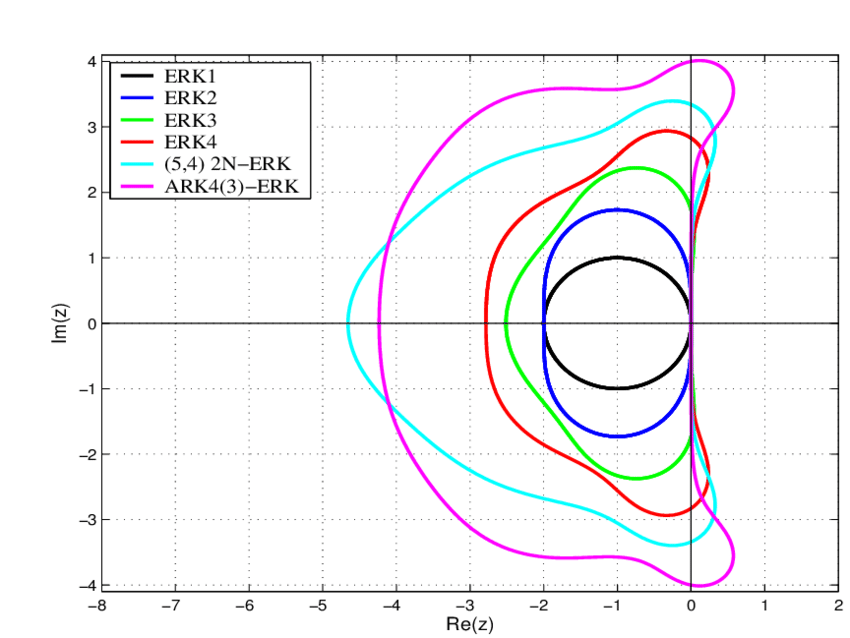
\includegraphics[width=0.7\textwidth]{images/stable.png}
			\caption{Stability Region \cite{article}}
		\end{figure}
	
	\section*{Number 5 c)}
		To pick the time step, $|\sigma \leq 1|$ and the following can be calculated. From the previous problem, the wave equation can't use the explicit euler scheme. For the 1d heat equation. 
		$$\frac{4\nu \Delta t}{(\Delta x)^2} \leq 2 $$
		$$ \makebox{\fbox{ \Delta t \leq \frac{(\Delta x)^2}{2} } } } $$
			
	
	\clearpage
	
	\section*{Appendix)}
		\subsection*{ Python Code for 1 a) }
			\lstinputlisting[language=Python]{HW1N1a.py}
		\subsection*{ Python Code for 2 a) }
			\lstinputlisting[language=Python]{HW1N2a.py}
		\subsection*{ Python Code for 3 a) }
			\lstinputlisting[language=Python]{HW1N3a.py}
		\subsection*{ Python Code for 3 b) }
			\lstinputlisting[language=Python]{HW1N3b.py}
		\subsection*{ Python Code for 4 }
			\lstinputlisting[language=Python]{HW1N4v2.py}
		\subsection*{ Python Code for 5 }
			\lstinputlisting[language=Python]{HW1N5.py}
			
	\printbibliography
		
\end{document}
